\documentclass[12pt]{article}
\usepackage[margin=1in]{geometry}
\usepackage{amsmath}
\usepackage{amssymb}
\usepackage{setspace}
\usepackage{graphicx}
\usepackage{cite}

\onehalfspacing

\title{Natural Computing Assessment}
\author{Exam Nos. B156771, [insert exam number here]}

\begin{document}
\maketitle
\section{Neural Network Training with PSO}
\subsection{Choosing the Fitness Function}
This task is interpreted to mean that we are to design a fitness function to evaluate the fitness of the network as a whole after it has been trained. In this sense, a clear component of this function must include the training and testing error in some fashion. We will denote the training error $e_T$, and the testing error $e_\tau$. Taking the average of the two would appear to be a sensible, if not standard course of action. However, a fitness function would need to incorporate a measure of how overfit the model is to the training data in order to be effective. In this sense, adding the difference between the two values is simple and effective. Ultimately, the fitness function takes the following form:
\begin{equation}
    f(e_T, e_\tau) = \frac{e_T + e_\tau}{2} + \left(e_\tau - e_T\right),
\end{equation}
where the error is calculated using the Mean Squared Error function.

\subsection{Defining the Search Space}
The search space of a PSO is given by $[a,b]^D$, where $a,b\in \mathbb{R}$, and $D\in\mathbb{N}$ is the dimension of the space. 
We will start by determining the value for $D$.
We define the shape of a neural network by a sequence $(a_n)_{n=1}^{l}$ where $l\in\mathbb{N}$ defines the number of layers, and each $a_n \in \mathbb{N}$ gives the number of neurons in layer $n$. 
The dimension of the weight vector for a would be the number of edges connecting each sequential pair of layers, plus the biases, given by the number of neurons in the latter of the pair of layers. Succinctly, the dimension $D$ of the search space is given by,
\begin{equation}
    D = \left(\sum_{i=1}^{l-1} a_{n+1}\left(a_n + 1\right)\right) - a_l,
\end{equation}
where the final decrement addresses non-existent bias terms in the output layer that were counted in the summation.

For this task, we set the shape to be $\left(6, 8, 1\right)$, meaning that the dimension of the search space $D=43$. 
To ensure that we are notified of a divergent swarm, we set $-a=b=20$, meaning that the search space for the PSO will be $\left[-20,20\right]^{43}$. 

\subsection{Training the Model}
For this task we trained two neural networks: one using Particle Swarm as its optimiser, and another using Stochastic Gradient Descent.
The model using SGD provides a fairly standard baseline on which to test the PSO model. 
In the code provided, the PSO neural net does not use any third party machine learning libraries as due to the nature of PSO, these neural nets only needed to consider forward propagation, not backwards.
For the SGD optimised net, Pytorch was used due to the myriad of material online explaining how to code it. 

Each network was trained with 10-fold cross validation using the cross-validate program provided (refer to the README in the task-1 directory on how to use it). 
The parameters for the PSO were as follows: $n=10$, $\omega=0.6$, $\alpha_1 = \alpha_2 = 1.61$. 
The parameters for the SGD were as follows: learning rate $=0.03$, momentum = $0.4$.
The figure below shows the training and testing loss of both over time:

\begin{figure}[h]                   
      \begin{center}                  
          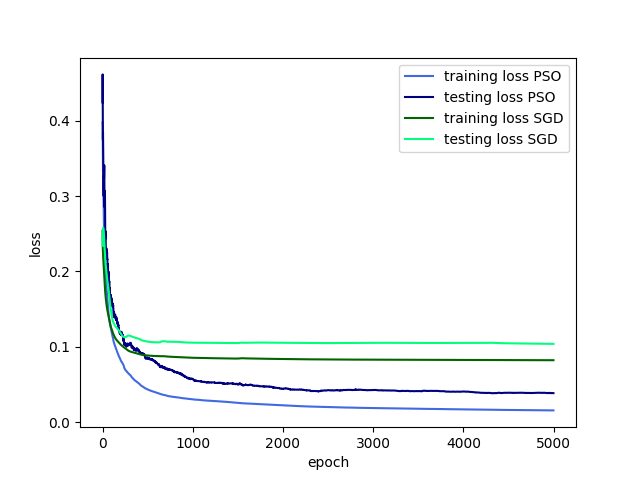
\includegraphics[scale=0.75]{/home/alexander/school/natural_computing/task-1/data/figures/nonlinear.png}    
      \end{center}                                                                                              
\end{figure}
The table below shows the final average training and testing losses, as well as the average fitness using equation (1):
\begin{center}
 \begin{tabular}{||c c c c||} 
 \hline
 Optimiser & Average Training Loss & Average Testing Loss & Average Fitness \\ [0.5ex] 
 \hline\hline
 PSO & 0.0159 & 0.0378 & 0.0489 \\ 
 \hline
 SGD & 0.0828 & 0.1164 & 0.1332 \\
 \hline
\end{tabular}
\end{center}

By these results it would appear that the model trained using PSO as its optimiser performed significantly better than the model trained with SGD. 
In a way, this could almost be expected. Gradient Descent follows the single path of a point gradually moving along the steepest descent in the search space.
In contrast, Particle Swarm has several particles searching for the (ideally) global, if not various local minima. 
This means that PSO is more likely to find a global minimum than SGD is, though how much more likely is still to be determined.
One benefit of SGD; however, is how quickly it converges to the minimum. 
We can see by figure 1 that the SGD model reached a stable training and test loss much quicker than its PSO counterpart, which can have its benefits depending on the application of the model.
Nevertheless, it is clear that for our purposes the PSO is superior. 
While it was slower to train, the low loss on both the training and testing sets for each fold of the cross validation demonstrates that it is well suited for neural network training. Furthermore, by eliminating backpropagation as a consideration in training, developing the model is conceptually simpler as well. 
\subsection{Restriction to Linear Inputs}
\subsection{Particle Swarm or Gradient Descent}
\end{document}
